% ******************************* PhD Thesis Template **************************
% Please have a look at the README.md file for info on how to use the template

\documentclass[a4paper,12pt,times,numbered,print,index]{PhDThesisPSnPDF}

% ******************************************************************************
% ******************************* Class Options ********************************
% *********************** See README for more details **************************
% ******************************************************************************

% `a4paper'(The University of Cambridge PhD thesis guidelines recommends a page
% size a4 - default option) or `a5paper': A5 Paper size is also allowed as per
% the Cambridge University Engineering Deparment guidelines for PhD thesis
%
% `11pt' or `12pt'(default): Font Size 10pt is NOT recommended by the University
% guidelines
%
% `oneside' or `twoside'(default): Printing double side (twoside) or single
% side.
%
% `print': Use `print' for print version with appropriate margins and page
% layout. Leaving the options field blank will activate Online version.
%
% `index': For index at the end of the thesis
%
% `draftclassic': For draft mode without loading any images (same as draft in book)
%
% `draft': Special draft mode with line numbers, images, and water mark with
% timestamp and custom text. Position of the text can also be modified.
%
% `abstract': To generate only the title page and abstract page with
% dissertation title and name, to submit to the Student Registry
%
% `chapter`: This option enables only the specified chapter and it's references
%  Useful for review and corrections.
%
% ************************* Custom Page Margins ********************************
%
% `custommargin`: Use `custommargin' in options to activate custom page margins,
% which can be defined in the preamble.tex. Custom margin will override
% print/online margin setup.
%
% *********************** Choosing the Fonts in Class Options ******************
%
% `times' : Times font with math support. (The Cambridge University guidelines
% recommend using times)
%
% `fourier': Utopia Font with Fourier Math font (Font has to be installed)
%            It's a free font.
%
% `customfont': Use `customfont' option in the document class and load the
% package in the preamble.tex
%
% default or leave empty: `Latin Modern' font will be loaded.
%
% ********************** Choosing the Bibliography style ***********************
%
% `authoryear': For author-year citation eg., Krishna (2013)
%
% `numbered': (Default Option) For numbered and sorted citation e.g., [1,5,2]
%
% `custombib': Define your own bibliography style in the `preamble.tex' file.
%              `\RequirePackage[square, sort, numbers, authoryear]{natbib}'.
%              This can be also used to load biblatex instead of natbib
%              (See Preamble)
%
% **************************** Choosing the Page Style *************************
%
% `default (leave empty)': For Page Numbers in Header (Left Even, Right Odd) and
% Chapter Name in Header (Right Even) and Section Name (Left Odd). Blank Footer.
%
% `PageStyleI': Chapter Name next & Page Number on Even Side (Left Even).
% Section Name & Page Number in Header on Odd Side (Right Odd). Footer is empty.
%
% `PageStyleII': Chapter Name on Even Side (Left Even) in Header. Section Number
% and Section Name in Header on Odd Side (Right Odd). Page numbering in footer

% Uncomment to change page style
%\pagestyle{PageStyleII}

% ********************************** Preamble **********************************
% Preamble: Contains packages and user-defined commands and settings
% ******************************************************************************
% ****************************** Custom Margin *********************************

% Add `custommargin' in the document class options to use this section
% Set {innerside margin / outerside margin / topmargin / bottom margin}  and
% other page dimensions
\ifsetCustomMargin
  \RequirePackage[left=37mm,right=30mm,top=35mm,bottom=30mm]{geometry}
  \setFancyHdr % To apply fancy header after geometry package is loaded
\fi

% Add spaces between paragraphs
%\setlength{\parskip}{0.5em}
% Ragged bottom avoids extra whitespaces between paragraphs
\raggedbottom
% To remove the excess top spacing for enumeration, list and description
%\usepackage{enumitem}
%\setlist[enumerate,itemize,description]{topsep=0em}

% *****************************************************************************
% ******************* Fonts (like different typewriter fonts etc.)*************

% Add `customfont' in the document class option to use this section

\ifsetCustomFont
  % Set your custom font here and use `customfont' in options. Leave empty to
  % load computer modern font (default LaTeX font).
  %\RequirePackage{helvet}
\usepackage{fontspec}
\setmainfont{Latin Modern}
  % For use with XeLaTeX
  %  \setmainfont[
  %    Path              = ./libertine/opentype/,
  %    Extension         = .otf,
  %    UprightFont = LinLibertine_R,
  %    BoldFont = LinLibertine_RZ, % Linux Libertine O Regular Semibold
  %    ItalicFont = LinLibertine_RI,
  %    BoldItalicFont = LinLibertine_RZI, % Linux Libertine O Regular Semibold Italic
  %  ]
  %  {libertine}
  %  % load font from system font
  %  \newfontfamily\libertinesystemfont{Linux Libertine O}
\fi

% *****************************************************************************
% **************************** Custom Packages ********************************

% ************************* Algorithms and Pseudocode **************************

%\usepackage{algpseudocode}


% ********************Captions and Hyperreferencing / URL **********************

% Captions: This makes captions of figures use a boldfaced small font.
%\RequirePackage[small,bf]{caption}

\RequirePackage[labelsep=space,tableposition=top]{caption}
\renewcommand{\figurename}{Fig.} %to support older versions of captions.sty


% *************************** Graphics and figures *****************************

%\usepackage{rotating}
%\usepackage{wrapfig}

% Uncomment the following two lines to force Latex to place the figure.
% Use [H] when including graphics. Note 'H' instead of 'h'
%\usepackage{float}
%\restylefloat{figure}

% Subcaption package is also available in the sty folder you can use that by
% uncommenting the following line
% This is for people stuck with older versions of texlive
%\usepackage{sty/caption/subcaption}
\usepackage{subcaption}

% ********************************** Tables ************************************
\usepackage{booktabs} % For professional looking tables
\usepackage{multirow}

%\usepackage{multicol}
%\usepackage{longtable}
%\usepackage{tabularx}


% *********************************** SI Units *********************************
\usepackage{siunitx} % use this package module for SI units


% ******************************* Line Spacing *********************************

% Choose linespacing as appropriate. Default is one-half line spacing as per the
% University guidelines

% \doublespacing
% \onehalfspacing
% \singlespacing


% ************************ Formatting / Footnote *******************************

% Don't break enumeration (etc.) across pages in an ugly manner (default 10000)
%\clubpenalty=500
%\widowpenalty=500

%\usepackage[perpage]{footmisc} %Range of footnote options


% *****************************************************************************
% *************************** Bibliography  and References ********************

%\usepackage{cleveref} %Referencing without need to explicitly state fig /table

% Add `custombib' in the document class option to use this section
\ifuseCustomBib
   \RequirePackage[square, sort, numbers, authoryear]{natbib} % CustomBib

% If you would like to use biblatex for your reference management, as opposed to the default `natbibpackage` pass the option `custombib` in the document class. Comment out the previous line to make sure you don't load the natbib package. Uncomment the following lines and specify the location of references.bib file

%\RequirePackage[backend=biber, style=numeric-comp, citestyle=numeric, sorting=nty, natbib=true]{biblatex}
%\addbibresource{References/references} %Location of references.bib only for biblatex, Do not omit the .bib extension from the filename.

\fi

% changes the default name `Bibliography` -> `References'
\renewcommand{\bibname}{References}


% ******************************************************************************
% ************************* User Defined Commands ******************************
% ******************************************************************************

% *********** To change the name of Table of Contents / LOF and LOT ************

%\renewcommand{\contentsname}{My Table of Contents}
%\renewcommand{\listfigurename}{My List of Figures}
%\renewcommand{\listtablename}{My List of Tables}


% ********************** TOC depth and numbering depth *************************

\setcounter{secnumdepth}{2}
\setcounter{tocdepth}{2}


% ******************************* Nomenclature *********************************

% To change the name of the Nomenclature section, uncomment the following line

%\renewcommand{\nomname}{Symbols}


% ********************************* Appendix ***********************************

% The default value of both \appendixtocname and \appendixpagename is `Appendices'. These names can all be changed via:

%\renewcommand{\appendixtocname}{List of appendices}
%\renewcommand{\appendixname}{Appndx}

% *********************** Configure Draft Mode **********************************

% Uncomment to disable figures in `draft'
%\setkeys{Gin}{draft=true}  % set draft to false to enable figures in `draft'

% These options are active only during the draft mode
% Default text is "Draft"
%\SetDraftText{DRAFT}

% Default Watermark location is top. Location (top/bottom)
%\SetDraftWMPosition{bottom}

% Draft Version - default is v1.0
%\SetDraftVersion{v1.1}

% Draft Text grayscale value (should be between 0-black and 1-white)
% Default value is 0.75
%\SetDraftGrayScale{0.8}


% ******************************** Todo Notes **********************************
%% Uncomment the following lines to have todonotes.

%\ifsetDraft
%	\usepackage[colorinlistoftodos]{todonotes}
%	\newcommand{\mynote}[1]{\todo[author=kks32,size=\small,inline,color=green!40]{#1}}
%\else
%	\newcommand{\mynote}[1]{}
%	\newcommand{\listoftodos}{}
%\fi

% Example todo: \mynote{Hey! I have a note}

% ******************************** Highlighting Changes **********************************
%% Uncomment the following lines to be able to highlight text/modifications.
%\ifsetDraft
%  \usepackage{color, soul}
%  \newcommand{\hlc}[2][yellow]{{\sethlcolor{#1} \hl{#2}}}
%  \newcommand{\hlfix}[2]{\texthl{#1}\todo{#2}}
%\else
%  \newcommand{\hlc}[2]{}
%  \newcommand{\hlfix}[2]{}
%\fi

% Example highlight 1: \hlc{Text to be highlighted}
% Example highlight 2: \hlc[green]{Text to be highlighted in green colour}
% Example highlight 3: \hlfix{Original Text}{Fixed Text}

% *****************************************************************************
% ******************* Better enumeration my MB*************
\usepackage{enumitem}

% ************************ Thesis Information & Meta-data **********************
% Thesis title and author information, refernce file for biblatex
% ************************ Thesis Information & Meta-data **********************
%% The title of the thesis
\title{Rest API in Digital Infrastructures of the Greek Government}
%\texorpdfstring is used for PDF metadata. Usage:
%\texorpdfstring{LaTeX_Version}{PDF Version (non-latex)} eg.,
%\texorpdfstring{$sigma$}{sigma}

%% Subtitle (Optional)
\subtitle{}

%% The full name of the author
\author{Michail Loukeris}

%% Department (eg. Department of Engineering, Maths, Physics)
\dept{Department of Management Science and Technology}

%% University and Crest
\university{Athens University of Economics and Business}
% Crest minimum should be 30mm.
\crest{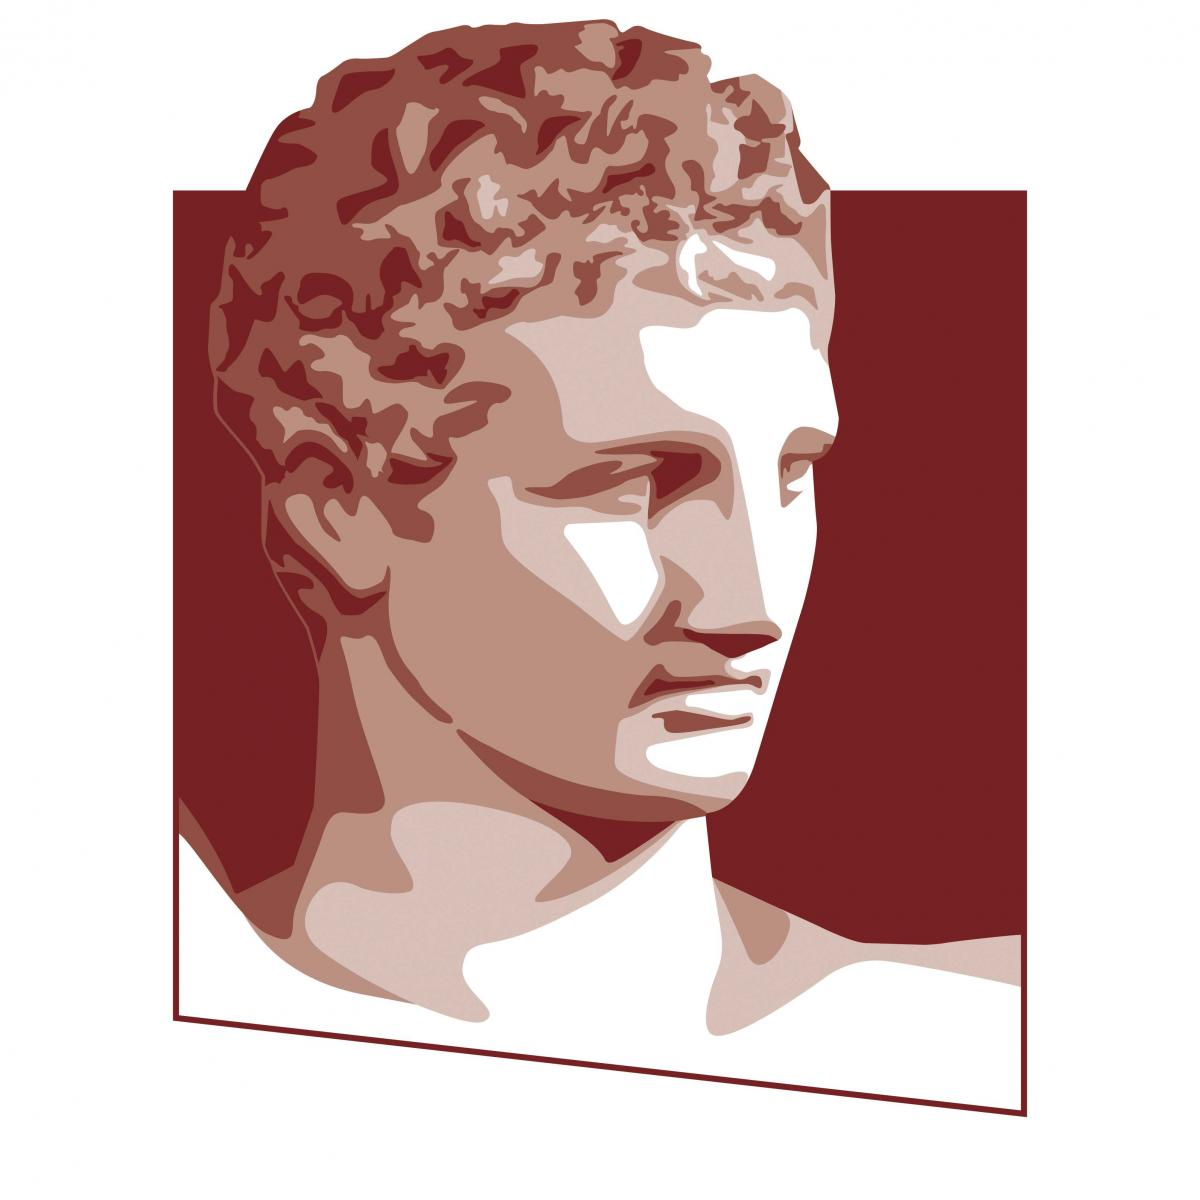
\includegraphics[width=0.2\textwidth]{University_Crest}}
%% Use this crest, if you are using the college crest
%% Crest long miminum should be 65mm
%\crest{\includegraphics[width=0.45\textwidth]{University_Crest_Long}}

%% College shield [optional] 
% Crest minimum should be 30mm.
%\collegeshield{\includegraphics[width=0.2\textwidth]{CollegeShields/Kings}}


%% Supervisor (optional)
%% for multiple supervisors, append each supervisor with the \newline command
\supervisor{Prof. P. Louridas}
%Prof. C.D. Supervisor}

%% Supervisor Role (optional) - Supervisor (default) or advisor
% \supervisorrole{\textbf{Supervisors: }}
%% if no title is desired:
% \supervisorrole{}

%% Supervisor line width: required to align supervisors
%\supervisorlinewidth{0.35\textwidth}

%% Advisor (optional)
%% for multiple advisors, append each advisor with the \newline command
%\advisor{Dr. A. Advisor\newline
%Dr. B. Advisor}
     
%% Advisor Role (optional) - Advisor (default) or leave empty
% \advisorrole{Advisors: }
%% if no title is required
% \advisorrole{}

%% Advisor line width: required to align supervisors
%\advisorlinewidth{0.25\textwidth}


%% You can redefine the submission text:
% Default as per the University guidelines:
% ``This dissertation is submitted for the degree of''
%\renewcommand{\submissiontext}{change the default text here if needed}

%% Full title of the Degree
\degreetitle{Management Science and Technology}

%% College affiliation (optional)
\college{}
	
% Submission date
% Default is set as {\monthname[\the\month]\space\the\year}
%\degreedate{September 2014} 

%% Meta information
\subject{LaTeX} \keywords{{LaTeX} {Bachelor Thesis} {Engineering} {Athens University of Economics and Business}}


% ***************************** Abstract Separate ******************************
% To printout only the titlepage and the abstract with the PhD title and the
% author name for submission to the Student Registry, use the `abstract' option in
% the document class.

\ifdefineAbstract
 \pagestyle{empty}
 \includeonly{Declaration/declaration, Abstract/abstract}
\fi

% ***************************** Chapter Mode ***********************************
% The chapter mode allows user to only print particular chapters with references
% Title, Contents, Frontmatter are disabled by default
% Useful option to review a particular chapter or to send it to supervisior.
% To use choose `chapter' option in the document class

\ifdefineChapter
 \includeonly{Chapter3/chapter3}
\fi

% ******************************** Front Matter ********************************
\begin{document}

\frontmatter

\maketitle

% ******************************* Thesis Dedidcation ********************************

\begin{dedication} 

I would like to dedicate this thesis to my loving parents \dots

\end{dedication}


% ******************************* Thesis Declaration ***************************

\begin{declaration}

I hereby declare that except where specific reference is made to the work of 
others, the contents of this dissertation are original and have not been 
submitted in whole or in part for consideration for any other degree or 
qualification in this, or any other university. This dissertation is my own 
work and contains nothing which is the outcome of work done in collaboration 
with others, except as specified in the text and Acknowledgements.

% Author and date will be inserted automatically from thesis.tex \author \degreedate

\end{declaration}


% ************************** Thesis Acknowledgements **************************

\begin{acknowledgements}      


And I would like to acknowledge ...

First and foremost,  my academic supervisor, Prof. Panagiotis Louridas
for supporting me during this semester by pointing me to the right
direction in choosing an interesting, both academically and practically,
topic for this thesis, as well as for his immediate support whenever I 
needed it. As well as Prof. Diomidis Spinellis for teaching me what a good
research paper looks like.

I would also like to show gratitude to all my colleagues in GRNET,
who treated me first as a friend, and taught me all I know when it comes to
recruiting and selecting employees. Moreover, I would like to point out Ntora Morfi
and George Korfiatis from GRNET and thank them for trusting me and bringing me onboard
to their organization.

Finally, I would like to thank my family and friends.
Without their patience, encouragement and support all these four years of my studies,
this paper would have never been accomplished.


\end{acknowledgements}

% ************************** Thesis Abstract *****************************
% Use `abstract' as an option in the document class to print only the titlepage and the abstract.
\begin{abstract}
	 
Recent technological developments strongly influence the way we lead our every - day life and the way we perform daily activities as shopping and communication. More and more new users are getting access to the Internet and to the newest technological tools, in order to make their life easier and better.

Having perceived the advantages of the use of new technology tools, many Governments worldwide have consistently, for the last twenty years, introduced new tools into state operational structure, in order to simplify their public services, make them widely accessible to the public, reduce the red tape, offer more efficient services and therefore a more effective governance. Countries, like Estonia, the UK, Singapore and Denmark have successfully established fully digitalised public services, including tax paying, transportation, drive licence issuing, and employment procedures.

This research set out to explore the Application Programming Interface (API) landscape in the EU public sector and how APIs could play a role into the digital transformation of governance.  More specifically, the aim of this work has been to examine the ability of Web APIs (hereafter “APIs”) to assist Member States of the EU into enabling their digital transformation. Areas of specific focus include cross-border interoperability between Member States and the opportunity for the EU to become involved in developing or advocating API standards.

From a technological point of view Application Programming Interface (API) refers to a set of clearly defined methods of communication between a service and any other software or components. It is essentially a software intermediary that allows two applications to interact with each other. In the public sector, APIs enable important functionality and information held in one agency’s system or department to be readily available to another without significant and expensive development effort. As well as cross-departmental (agency) access to functionality and information (or even cross-border with a different country’s administration) APIs also provide the ability to share information and functionality more widely, i.e. to developers and ultimately to citizens for consumption through web or mobile based applications. 

As APIs enable the public sector to create ‘ecosystems’ inside and outside a government system, overcome the restrictions of traditional integration solutions, facilitate the opening of large data sources to citizens and other third parties and support innovation, they seem to play a key role in the digital transformation of efficient governance, generating benefits for the citizen, for business and for the economy.


\end{abstract}


% *********************** Adding TOC and List of Figures ***********************

\tableofcontents

\listoffigures

\listoftables

% \printnomenclature[space] space can be set as 2em between symbol and description
%\printnomenclature[3em]

\printnomenclature

% ******************************** Main Matter *********************************
\mainmatter

%!TEX root = ../thesis.tex
%*******************************************************************************
%*********************************** First Chapter *****************************
%*******************************************************************************

\chapter{Introduction}  %Title of the First Chapter

\ifpdf
    \graphicspath{{Chapter1/Figs/Raster/}{Chapter1/Figs/PDF/}{Chapter1/Figs/}}
\else
    \graphicspath{{Chapter1/Figs/Vector/}{Chapter1/Figs/}}
\fi

At a strategy level, the Tallinn Declaration, signed on the 6th October 2017
~\citep{tallin_declaration}, confirms the commitment to the vision set out in the EU eGovernment
Action Plan 2016-2020~\citep{action_plan} and in the European Interoperability Framework (EIF)~\citep{eif}.
In a time span of five years (2018-2022), steps will be taken towards
the implementation of the following principles in EU open organizations: “computerized
naturally, comprehensiveness furthermore, availability”, “once-just”, “dependability
and security", “transparency and straightforwardness”, and “interoperability as a
matter of course”, just as national interoperability structures dependent on the
European Interoperability Framework (EIF).

In the Declaration the “user-centricity principles for design and delivery of
digital public services” is vital. Public administrations and digital public services,
upon interaction must fulfill the following requirements: digital interaction, accessibility, security, availability
and usability, reduction of the administrative burden, digital delivery of public services,
citizen engagement, incentives for digital service use, protection of personal data and
privacy, redress and complaint mechanisms. At the same time, the Communication on “Building the data economy” (COM (2017) 9)
looks at proven or potential blockages to the free movement of data and presents
options to remove unjustified and/or disproportionate data location restrictions
in the EU. It also considers the barriers around access to, and transfer of,
non-personal machine-generated data and data liability, as well as issues related
to the portability of non-personal data, interoperability and standards.
In particular, it aims at the development of technical solutions for
the reliable exchange and identification of data. 

Moreover, the digital transformation of society, business and government is raising
issues for a range of policy matters in the EU. As e-government has
been in place for the last 20 years is several EU countries including the UK, Estonia etc.,
it is timely to explore the interaction between
technology and government activities from the perspective of digital government.

Aspects of the digital
transformation of government concern the use of web Application Programming Interfaces
(hereafter called “APIs”)). APIs can be seen as “safe entry ports for new and
innovative uses of data” held by companies and potentially, public administrations.

This study is set to explore
web APIs as enablers for the digital transformation of governments. While
digital transformation of government is much wider than the technologies which
can potentially support it, an analysis of the role of APIs in the public sector
is highly relevant to illustrate how technology can enable transformation of
government. This study examines APIs, and their role in the EU public sector as
well as it points out the differences with the private sector and explores future
trends with a particular focus on current use of APIs in projects developed by various
EU Countries. Specifically, in the first chapter we present a glossary as well as an API
overview. Next, we discuss APIs as means to create ecosystems in the public sector and
to overcome complex integration. We analyze how it supports open government initiatives and
how it promotes innovation as well as some challenges and considerations along with some
quantitative metrics. Once we cover all the above we will explore the differences of the public 
with the private sector in terms of API usage and more specifically we will talk about API availability, business models and disruption as well as making money from APIs. Finally,
we will have a look at future API trends. The final chapter includes my internship report.

\clearpage

%********************************** %First Section  **************************************
\section{Glossary} %Section - 1.1 

% Note: It may be necessary to compile the document several times to get a multi-page table to line up properly
\begin{longtable}[c]{|l|l|}
	\hline
	\multicolumn{1}{|c|}{\textbf{Term}} & \multicolumn{1}{c|}{\textbf{Definition}} \\ \hline
	\endfirsthead
	%
	\endhead
	%
	API & \begin{tabular}[c]{@{}l@{}}Application Programming Interface — It is a set of clearly\\ defined methods of communication between the service\\ and any other software or components.\end{tabular} \\ \hline
	API Ecosystem & \begin{tabular}[c]{@{}l@{}}The developers, and the users of the application constructs\\ they build through an API, either within a company or on\\ the Internet with business partners, customers, citizens etc.\end{tabular} \\ \hline
	API Economy & \begin{tabular}[c]{@{}l@{}}A set of business models and channels — based on secure\\ access of functionality and exchange of data to an ecosystem\\ of developers and the users of the app constructs they\\ build — through an API, either within a company or on the\\ Internet with business partners, customers, citizens etc.\end{tabular} \\ \hline
	API Versioning & \begin{tabular}[c]{@{}l@{}}The ability to change without rendering older versions of\\ the same API inoperable.\end{tabular} \\ \hline
	\begin{tabular}[c]{@{}l@{}}API\\ Standardisation\end{tabular} & \begin{tabular}[c]{@{}l@{}}A uniform way for APIs to be expressed and consumed,\\ from COM and CORBA object brokers to web services\\ to today’s RESTful patterns.\end{tabular} \\ \hline
	\begin{tabular}[c]{@{}l@{}}API information\\ control\end{tabular} & \begin{tabular}[c]{@{}l@{}}A built-in means for enriching and handling the\\ information embodied by the API. This information\\ includes metadata, approaches to handling batches of\\ records, and hooks for middleware platforms, message\\ brokers, and service buses. It also defines how APIs\\ communicate, route, and manipulate the information\\ being exchanged.\end{tabular} \\ \hline
	API portal & \begin{tabular}[c]{@{}l@{}}A means for developers to discover, collaborate,\\ consume, and publish APIs. To support the overall\\ goal of self-service, these portals describe APIs in\\ a way that represents their functionality, context\\ (the business semantics of what they do, and how \\ they do it), non-functional requirements (scalability,\\ security, response times, volume limits, and resiliency\\ dimensions of the service), versioning, and metrics \\ tracking usage, feedback, and performance.\\ For organizations without mature master data or\\ architectural standards, the API portal can still offer\\ visibility into existing APIs and provide contact information\\ for individuals who can describe features, functions, and\\ technical details of services.\end{tabular} \\ \hline
	API gateway & \begin{tabular}[c]{@{}l@{}}A mechanism that allows consumers to become\\ authenticated and to “contract” with API specifications\\ and policies that are built into the API itself. Gateways\\ make it possible to decouple the “API proxy”—the node\\ by which consumers logically interact with the service—from\\ the underlying application for which the actual service is \\ being implemented. The gateway layer may offer the means\\ to load balance and throttle API usage.\end{tabular} \\ \hline
	API brokers & \begin{tabular}[c]{@{}l@{}}Enrichment, transformation, and validation services\\ to manipulate information coming to/from APIs, as\\ well as tools to embody business rule engines, workflow,\\ and business process orchestration on top of underlying APIs.\end{tabular} \\ \hline
	\begin{tabular}[c]{@{}l@{}}API\\ management\\ and monitoring\end{tabular} & \begin{tabular}[c]{@{}l@{}}A centralized and managed control level that provides\\ monitoring, service level management, \\System Development Life Cycle (SDLC) process\\ integration, and role-based access management across\\ all three layers above. It includes the ability to instrument\\ and measure API usage, and even capabilities to price and\\ bill charge-back based on API consumption—to internal,\\ or potentially external, parties.\end{tabular} \\ \hline
	RESTful API & \begin{tabular}[c]{@{}l@{}}REST stands for “representational state transfer.” APIs\\ built according to REST architectural standards are\\ stateless and offer a simpler alternative to some SOAP\\ standards. For example, REST enables plain-text exchanges\\ of data assets instead of using complex WSDL protocols which \\ is an XML format for describing network services as a set \\of endpoints operating on messages containing either\\ document-oriented or procedure-oriented information.\\ It also makes it possible to inherit security policies\\ from an underlying transport mechanism. At a high level,\\ these and other simplified approaches can deliver better\\ performance and faster paths to develop, deploy, and\\ triage.\end{tabular} \\ \hline
	\caption{Glossary}
	\label{glossary}\\
\end{longtable}

%********************************** %Second Section  *************************************
\section{API Overview} %Section - 1.2


APIs have become a key technological component of modern digital
architectures, impacting every sector of the global economy. In the public
sector specifically, APIs are a fundamental enabler of the transformation of its
operations from analog (manual, paper) to digital.

The purpose of this study is to showcase the 
major contribution of APIs, when member states are in
pursuit of their digital transformation.
In order to explore this purpose, our investigation has
covered the following topics:

\begin{itemize}
	\item The current use of APIs in the EU public sector.
	\item Differences between API use in the public and the private sector.
	\item The future trends for APIs.
	\item Aspects of the API Landscape including API Ecosystems, API as low complexity infrastructures,
	API as components of a business plan.
\end{itemize}
                                                                       
In summary, in this study web — based research has been used as well as my
experience from my internship in GRNET to gather information for analysis
of successful but diverse API based case studies from a range of EU countries
and sectors.

\subsection{API Overview}



API interaction occurs when one application would like to:
\begin{itemize}
	\item Request a service from another application.
	\item Send data to that application.
	\item Access or query the data held by another application.
	\item Update data held in that application.

\end{itemize}

\subsubsection{Types of APIs}

APIs represent an architectural approach that revolves around providing
programmable interfaces to different applications. It is technology agnostic,
and creates a flexible, loosely coupled architecture that allows a solution to be
made up of components that can more easily be switched in and out. The API approach
is also a essential enabler for application developers to create apps that rapidly adapt
to end user needs~\citep{hcl_tech}. 

In the public sector, APIs enable important functionality and information held in
one agency’s system or department to be readily available to another without
significant and expensive development effort. As well as cross-departmental
access to functionality and information (or even cross-border with a
different country’s administration) APIs also provide the ability to share
information and functionality more widely, i.e., to developers and ultimately
to citizens for consumption through web or mobile based applications.

Although there are many different types of API (see Appendix I), this study is
most concerned with web APIs. Web services expose these APIs as endpoints that
any internet-enabled language or software can access, in exactly the same way
browsers access websites and services~\citep{fed_tech}. Web APIs deliver requests to the
service provider, and then deliver the response back to the requestor,
i.e., they are an interface for web applications, or applications that need to
connect to each other via the Internet to communicate~\citep{define_api}.

Web APIs themselves can be broken down further based on the type of data format
that they harness, for example, well known types are Simple Object Access Protocol
(SOAP), Remote Procedure Call (RPC) based APIs, and the Representational State
Transfer (REST) architectural style. GraphQL – is a data query language growing
in popularity and has been adopted by leading social media outlets such as Facebook
and Pinterest~\citep{graphql} as a type of API. While typical REST APIs require loading
from multiple URLs, GraphQL APIs get all the data an app developer needs in a single
request enhancing speed of response even on slow mobile network connections~\citep{graphql}.

Whilst the more traditional APIs are used as integration points within systems
hidden from view, Web APIs are often publicly available and can be ‘advertised’
via API Directory sites online. Tens of thousands~\citep{programmableweb_search} are available for developers
to deliver consumable information to end users to do everything, from checking
traffic and weather, to updating a social media status, or even to make payments.

\subsubsection{API Standards}

In the geospatial domain, besides existing private companies famous API proposals
(e.g. Google Map), the Open Geospatial Consortium (OGC) has created standards to
support the exchange of geospatial information~\citep{opengeospatial}. They describe their Web services
API standards as an agreed specification of rules and guidelines about how to
implement software interfaces and data encodings~\citep{opengeospatial_elearning}. Geospatial software vendors,
developers and users collaborate in the OGC’s consensus process to develop and
agree on standards that enable information systems to exchange geospatial
information and instructions for geoprocessing. OGC standards are open standards.
The OGC interface standards are also available in the REST style, and cover a
number of aspects:
\begin{itemize}
	\item Visualisation standards e.g. Web Map Service (WMS).
	\item Data Access Standards e.g. Web Feature Service (WFS), SensorThings API.
	\item Processing Standards e.g. Web Processing Service (WPS).
	\item Metadata and Catalogue Service Standards e.g. Catalog Service for the Web (CWS).
	\item The informatics contract between the client code which manipulates normalized
	data structures of geographic information based on the published API and the library
	code, e.g. the GeoAPI Implementation Standard.
\end{itemize}

The standards above are part of the few globally agreed specifications adopted by
the Technical Committee 211 of the International Organization for Standardization
(ISO). ISO is also known to be working on standards in other sectors, notably in
Financial Services with ISO 20022~\citep{iso}: however, because of they are work in
progress,
details about them are still limited. Whilst standards of this formal and specific
nature are used in the EU, there is clear evidence that the need for harmonizing
APIs lifecycle has been recognized. For example, the UK Government Digital Service
recognized that departments were developing APIs using different tools, platforms
and approaches~\citep{tech_gov}, and have set about working with industry to create a set of
common principles for API design. The output has been a set of guidelines on how
developers working in any UK public sector organisation should build APIs~\citep{gov_uk_api} to
ensure consistency, and success. These guidelines apply to other countries too.
Although they are titled as a ‘standard’, they
are generic, and not exact or specific in the way that an ISO or OGC standard is.
Nevertheless, given the fact that government is increasingly using APIs to
automate processes and provide citizens with access to new services it is hoped
this approach will make integration simpler and faster.
%!TEX root = ../thesis.tex
%*******************************************************************************
%****************************** Second Chapter *********************************
%*******************************************************************************

\chapter{APIs in the Public Sector}

\ifpdf
    \graphicspath{{Chapter2/Figs/Raster/}{Chapter2/Figs/PDF/}{Chapter2/Figs/}}
\else
    \graphicspath{{Chapter2/Figs/Vector/}{Chapter2/Figs/}}
\fi

The Internet, social media, smartphones, and access to real-time information
have not only made people’s daily lives easier, but have changed citizens’
expectations of how products and services are delivered. In the public sector,
this shift has raised the expectations of citizens and business in their
interactions with government.

People are demanding transparency, accountability, access to information and
competent service delivery from their governments. They also expect policies
and services to be tailored to their needs and address their concerns.

In this section, we will explore how APIs are used in the public sector.
We will firstly look at typical uses, such as the enablement of ecosystems,
before looking at some specific examples of API use. In addition, we will
cover some challenges and considerations, and examine data on the APIs
advertised in one of the most respected API Directories, (ProgrammableWeb)
as a further indicator of the way APIs are used in the public sector.


\section{APIs enable the public sector to create ‘ecosystems’}

API based ecosystems can be defined as the extended interrelationships enabled
by developers who create applications that link various groups of stakeholders
to each other via API based solutions that use the internet to communicate [cite 18].

An ecosystem may be created within a government agency, between agencies, or
it may be wider reaching, for example between a government and another government
or between a government, their citizens, and potentially third party providers.


% arctext from Andrew code with modifications:
%Variables: 1: ID, 2:Style 3:box height 4: Radious 5:start-angl 6:end-angl 7:text {format along path} 
\def\arctext[#1][#2][#3](#4)(#5)(#6)#7{
	
	\draw[
	color=white,
	thick,
	line width=1.3pt,
	fill=#2
	]
	(#5:#4cm+#3) coordinate (above #1) arc (#5:#6:#4cm+#3)
	-- (#6:#4) coordinate (right #1) -- (#6:#4cm-#3) coordinate (below right #1) 
	arc (#6:#5:#4cm-#3) coordinate (below #1)
	-- (#5:#4) coordinate (left #1) -- cycle;
	\def\a#1{#4cm+#3}
	\def\b#1{#4cm-#3}
	\path[
	decoration={
		raise = -0.5ex, % Controls relavite text height position.
		text  along path,
		text ={#7},
		text align = center,        
	},
	decorate
	]
	(#5:#4) arc (#5:#6:#4);
}

%arcarrow, this is mine, for beerware purpose...
%Function: Draw an arrow from arctex coordinate specific nodes to another 
%Arrow start at the start of arctext box and could be shifted to change the position
%to avoid go over another box.
%Var: 1:Start coordinate 2:End coordinate 3:angle to shift from acrtext box  
\def\arcarrow[#1](#2)(#3)[#4]{
	\draw[thick,-,>=latex,color=#1,line width=1pt,shorten >=-2pt, shorten <=-2pt] 
	let \p1 = (#2), \p2 = (#3), % To access cartesian coordinates x, and y.
	\n1 = {veclen(\x1,\y1)}, % Distance from the origin
	\n2 = {veclen(\x2,\y2)}, % Distance from the origin
	\n3 = {atan2(\y1,\x1)} % Angle where acrtext starts.
	in (\n3-#4: \n1) -- (\n3-#4: \n2); % Draw the arrow.
}


\begin{figure}
	\begin{center}
	\begin{tikzpicture}[
	% Environment Cfg
	font=\sf    \scriptsize,
	% Styles
	myarrow/.style={
		thick,
		-latex,
	},
	Center/.style ={
		circle,
		fill=white,
		text=root,
		align=center,
		font =\footnotesize,
		inner sep=1pt,          
	},
	]
	
	% Drawing the center
	\node[Center](ROOT) at (0,0) {Governemnt \\ APIs};
	
	% Drawing the Tex Arcs
	
	% \Arctext[ID][box-style][box-height](radious)(start-angl)(end-angl){|text-styles| Text}
	% Node 1:   
	\arctext[N1][black][30pt](3)(270)(90){|\footnotesize\bf\color{white}| Private};
	%Sub 1:
	\arctext[N1S1][black][26pt](5)(270)(90){|\footnotesize\bf\color{white}| Agency Systems };

	%Node 2:
	\arctext[N2][black][30pt](3)(-90)(0){|\footnotesize\bf\color{white}| Open Secured};
	%Sub 1:
	\arctext[N2S1][black][26pt](5)(90)(65){|\footnotesize\bf\color{white}| Developer Networks};

	%Sub 2:
	\arctext[N2S2][black][26pt](5)(65)(30){|\footnotesize\bf\color{white}| Commercial Developers};

	%Sub 3:
	\arctext[N2S3][black][26pt](5)(30)(0){|\footnotesize\bf\color{white}| Partner Service Providers};

	%Sub 4: 
	\arctext[N2S4][black][26pt](5)(0)(-60){|\footnotesize\bf\color{white}| Governemnt Agencies};
	
	%Sub 5: 
	\arctext[N2S4][black][26pt](5)(-90)(-60){|\footnotesize\bf\color{white}| Business Unit Developers};
	
	%Node 3:
    \arctext[N3][black][30pt](3)(0)(90){|\footnotesize\bf\color{white}| Open Public};

	\end{tikzpicture}
\end{center}
\label{Figure 1}
\caption{Ecosystems enabled by government APIs} [cite 19]
\end{figure}

\clearpage

The figure above illustrates the way in which APIs are used, and the typical
ecosystem that they facilitate in the public sector.
\begin{itemize}
	\item Private – Agency Systems: These APIs are generally used to facilitate
	 the sharing of data between systems within an agency, avoiding the need
	 for complex point to point integration. They are not visible to any person
	 or body outside of the agency and are generally in the domain of the IT
	 department. An example maybe a link between an internal HR system and a
	 Payroll solution.
	 \item Open Public – At Large Developer Networks: Open APIs (i.e. you do
	 not require permission to access them) are the access point for developers
	 to access large public data sources such as a census information or other
	 similar statistical data, perhaps live sensor data from which to create
	 citizen-facing applications.
	 \item Open Public – Commercial Developers: As above, but developers who are
	 looking to gather freely available data for use, generally, in applications
	 that can be sold. They may add value by ‘mashing’ the data, i.e. combining
	 data on public transportation networks with location data available on an
	 individual’s smart phone to help the citizen make travel choices in real-time...
	 Because of this openness, third-party integration of software is not only easier
	 but less problematic. Developers have access to the API at all times, so they
	 can ensure that the two-way communication between assorted pieces of software
	 is correct, rather than having to guess at the appropriate methods to use.
	 
	 It is also worth noting the economic stimulation that this can bring. Transport
	 for London’s policy of working with major IT players (Google, Apple, Waze etc.)
	 but allowing their data to be available via the Open Government License has led
	 to the creation of additional economic activity in the order of £100m of direct
	 value and has enabled some 1,000 jobs [cite 20].
	 \item Open Public/Secured – Partner Service Providers: The APIs are open to
	 partners perhaps in the private sector which may include healthcare providers
	 for example, who in some member states are interested in sharing healthcare
	 records, or confirming eligibility for free or subsidized treatment based on
	 data held by a government agency.
	 \item Open Secured – Government Agencies: These APIs are available to other
	 government agencies and allow them to share data only once they have
	 authenticated. This supports many of the core tenets of digital government,
	 allowing agencies to collect data on a citizen only once, and then share it
	 securely. An example may involve the sharing of citizen data between say the
	 agency responsible for income and taxation, and those providing benefits in
	 order that eligibility could be confirmed. Please see later case studies
	 relating to Estonia X-Road, and Amsterdam City Data for more on this.
	 
	 Although not specifically mentioned in the diagram above, the ability to use
	 APIs is not constrained by sector or geographical boundaries. Open Secured
	 – Government Agencies could include an application to application link
	 between governments of different member states. A good example (explored
	 further later) would be the Estonian X-Road Platform which uses APIs to
	 share citizen’s healthcare information with Finland.
	 \item Open Secured – Business Unit Developers: Similar to the above, but
	 instead of basic inter-agency data sharing, in this case the data is being
	 consumed and then in some way supplemented in order to be useful by developers
	 within a government agency. They are used to create custom applications around
	 internal data assets for agency use.
\end{itemize}

In summary, the creation of an ‘ecosystem’ of providers and consumers fosters
openness and efficiency, and can also spawn the development of innovative service
models, some of which may lead to revenue generation for the agencies concerned
(for example mapping data [cite 21], or gazetteer data). Their ability to provide access
into the heart of government, in turn allows government to realise its objectives
of openness, and of delivering efficient, secure, transparent and interoperable
citizen centric services. The APIs are, therefore, a crucial technological
component, which will underpin empowering the evolution of public service delivery
models, enabling agencies to accelerate their transformation from eGovernment to
Digital Government.

\section{APIs enable public sector agencies to overcome complex integration}

Nearly all EU countries have developed their computing infrastructure over
many years, constructing a legacy of large, complex information systems featuring
interfaces to pass information from one system to another. The majority of these
interfaces were point to point and custom built to meet the needs of a particular
project or agency at a point in time. As the number of interfaces grew, so did the
maintenance burden; the inter-relationships and the data duplication leading to an
expensive, complex and inefficient architecture [cite 22]. In summary, these
“siloed”, legacy government systems and associated business processes increase
risk and exacerbate challenges in data sharing and service delivery across the
ecosystem.

APIs provide an opportunity, in effect a structural ‘workaround’, to enable the
information within these legacy systems to be exposed with comparably low complexity
and investment. They can be plugged into legacy systems of record such as ERP
systems [cite 23], or citizen facing records to make the data records directly
available, thus helping to bypass the complex interfaces of existing systems,
and allow data sharing to be accomplished more easily. This means that a
well-designed government ecosystem could help minimise the frequency that
citizens or businesses will have to provide the same information (Once Only
Principle, OOP).

A good EU example of where API infrastructure is currently being used to overcome
the restrictions of traditional integration solutions is Estonia’s X-Road Platform.
It allows citizens to provide common ‘private and sensitive’ information to public administrations only once, for example, marital status. The ecosystem also includes
private institutions such as banks who can have access in order to perform various
functions. X-Road is examined in more detail in the case studies section of this report.

\textbf{EU Example: ESTONIA X-ROADS PLATFORM}

“X-Road is the backbone of e-Estonia. Invisible yet crucial, it allows the
nation’s various public and private sector e-Service databases to link up and
function in harmony.” [cite 24]

X-Road is a government API framework developed by the Estonian government
and licensed under the MIT license. It is also used as a backbone of the Finnish
National Data Exchange Layer.Originally built for SOAP/XML web services, it now
extends to REST APIs. Rather than requiring governments to develop API management
directly, X-Road provides an API management layer, including an API gateway,
which is open-sourced and available to governments worldwide. [cite 25]

The X-Road solution includes a security server to provide identity and access
management for government API access. It also provides central monitoring of
API traffic. In addition to the management of APIs, it also provides an
aggregation layer in front of multiple databases. This facilitates the creation
and delivery of data access APIs.

Since each government service/agency has its own databases they all use X-Road
to securely communicate and share ‘private and sensitive’ data to protect the
‘once only’ principle of sharing data with government. The service also incorporates
many other sectors numbering over 900 organisations and enterprises including those
in the banking, health and utility sectors [cite 26]. Whilst they may use the platform to
perform functions such as identity verification, powerful use cases such as automated extraction of funds from bank accounts for those failing to keep up to date with
taxes are possible.

All that being said, the X-Road itself is a ‘very low level engineered application’
[cite 27]. Following certification, an organisation deploys an x-road gateway
so that it can hold secure private communications via APIs with other certified
organisations that are legally able to share data with it. As a collective toolset,
the e-Estonia services provide the government of Estonia and its partners,
including Finland, with a platform on which to innovate and use digital
transformation to deliver new services across the globe.

\section{APIs support the public sector open government initiatives}

Open Government can be defined as the opening up of government processes,
proceedings, documents and data for public scrutiny and involvement, and is
now considered as a fundamental element of a democratic society [cite 28].
The Open government initiative started in 2009 by Barak Obama [cite 29], after that,
numerous governments adopted open data initiatives. It is founded on the
belief that greater transparency and public participation can not only lead
to better policies and services, they can also promote public sector
integrity, which is essential to regaining the trust of citizens in the
neutrality and reliability of public administrations.

APIs have become synonymous with facilitating the opening of large data sources
to citizens and other third parties. The Open Government imperatives have meant
that API technology has been exploited outside of the ‘IT department’,
providing access into large open data stores so that developers and their
applications and websites can more easily consume it. When a government agency
publishes an API for their data set, they open up new and innovative ways to
access the data. A developer might create a mobile or web app to display the
data intuitively or allow simple queries or automatically generate charts.

The most relevant public sector that expose government datasets is The European
Data Portal [cite 30] (EDP).

\textbf{EU Example: European Data Portal (EDP)}

The EDP provides access to 79 different catalogues, most with tens of thousands of
open datasets provided my member state governments. The same site also provides
access to over 300 use cases (services or applications) that have been developed
using the open data sets available. Some of these applications have been created
using APIs to query the EDP.

The access to the Portal is provided by a machine-readable API which enables its
users to search, create, modify and delete metadata on the portal.31 APIs are
available both via the Comprehensive Knowledge Archive Network (CKAN) [cite 32] and
SPARQL [cite 33] endpoints.

\section{APIs enable the public sector to innovate}

APIs enable new innovative service models which better engage citizens and allow
for more efficient delivery of their services. These services no longer have to
be provided directly by the agency, partners and citizen developers can use
available data to enable new solutions. Smart Cities and the vast amount of data
produced by sensors supports the development of dynamic platforms and ecosystems
providing contextualized, real-time location-based data from IoT or crowdsourcing
to business partners and startups giving them opportunities to create new services
or improve existing ones.

Transport for London have delivered successful innovation based on API use.
Although other more innovative services are coming of age in areas such as
Smart Cities, this example is one of concrete success in enhancing efficiency
and citizen service delivery.

\textbf{EU Example: TRANSPORT FOR LONDON (TfL)}

At recent European conference34, Transport for London detailed the investment that
that they had made:
\begin{itemize}
	\item 200 data elements are made available through an API to some 12,000
	developers producing some 600 apps that 40\% of Londoners use.
	\item TfL has formed partnerships with major IT players such as Apple
	(for mobile payment, rental ofbikes), Twitter (for pushing alerts out),
	a two-way data-sharing agreement with Waze (enriching the app with data
	from the road network that TfL manages while benefiting from data collected
	through Waze) and Google (enriching the maps application with real-time data).
	\item The data can be consumed under the terms of the UK Open Government
	Licence with some minimal additions for free. This is done under a statutory
	requirement as part of UK legislation.Mechanisms are in place to ensure that
	consumption remains at an acceptable level. There is one single set of data
	at the base that are both consumed by TfL for its purposes and by third	party
	developers. Developers must give attribution to TfL for the fact that their
	app includes TfL data.
	\item In terms of creation of additional economic activity, it has been
	calculated that this policy	generates GBP 100m of direct value and has enabled
	some 1,000 jobs.
	\item For data acquired by a third party, e.g. Waze data, restrictions resulting
	from the partnership agreement apply.
	\item All data made available is data that TfL collects anyway for its own
	purposes. TfL is not collecting additional data merely to make available to
	third parties.
	\item Mashing data provided by TfL with privately-held data can bring additional
	insights (e.g. "Are	there correlations between rainfall and collisions involving cyclists?”).
\end{itemize}

\section{Challenges and Considerations}

For the most part, externally facing public sector APIs involve the movement
of data that is sensitive as it often, in some way, refers to information about
a citizen. This poses a number of consistent challenges for government:
\begin{itemize}
	\item Security – APIs expose data, services, and transactions in order to
	build new services. This inherently increases the permeability of an
	organisation’s network, which can expose new vulnerabilities for
	exploitation. Therefore, APIs must be appropriately secured to ensure data
	privacy and to ensure citizen confidence in the service delivery channel.
	APIs intended for access to public data must be protected from inappropriate
	use or abuse such as denial of service. A number of security solutions exist
	such as OAuth and Certificate based authentication, which are used in
	conjunction with a wider cyber security strategy and cryptography.
	\item Regulation – APIs play a significant role in the facilitation of
	government transparency. A recent EU ruling [cite 35] makes providing
	transparency into all IT services that will be used in technology projects
	a condition for receiving government funding, and it is more than likely
	that APIs are the core technology required to support the transparency
	principle.
	\item Further regulatory considerations which must be adhered to when
	sharing data through any type of interface are the General Data Privacy
	Regulation [cite 36] (GDPR), the Payment Services Directive	(PSD2) [cite 37]
	and the Public Sector Information Directive (PSI) [cite 38].
	\item Specifications or Standards - Standards for APIs are available in
	small pockets such as the OGC [cite 39]	standard, and the developing ISO
	standard in Financial Services [cite 40]. However, many organisations are developing
	APIs based on an agreed internal specification or style guide to promote
	consistency, rather than what might normally be recognised as a de facto
	‘standard’. Each API comes with detailed documentation for consumers which
	provides clarity on the type of API	(RESTful, GRAPHQL, GRPC etc.). There
	appears to be limited appetite for further standard	development in the
	aftermath of ‘Open Government’ which is different to the impact ‘Open Banking’
	has had in the EU which precipitated the agreement of an API standard (in the
	UK initially at least) [cite 41].
\end{itemize}

The work conducted by the FIWARE Foundation (Future Internet Ware) tries to
overcome some of the challenges listed above. FIWARE will be analysed later
in the document, but in summary it is funded by a combination of EU, corporate
membership and venture capital funding and has created a scalable open source
platform used to access and manage heterogeneous context information through
open APIs [cite 42]. A standard for exchange of context information: FIWARE-NGSI
(Next Generation Service Interface) is an open standard API to be used for Smart
Cities, Smart Industry and Smart Agrifood [cite 43]. The EU has noted its success to
date, however, its success in landing a standardized API that is universally
used will be known only in time.
\begin{itemize}
	\item Business Models – In the public sector, generating income from the
	provision of data that is publically owned, and is being used for the
	public good, has not led to the charging of users who wish to consume
	or query this type of data. Examples of charging mechanisms being in place
	are	limited, one being the UK’s Ordnance Survey maps [cite 44], and KLIP (one of
	the case studies explored later in the Section dedicated to the case studies)
	which charges map requestors to have a digital map of utility services
	generated for a specific location. 
\end{itemize}

\section{Quantitative assessment of API use in the public sector}

It is hard to realistically quantify the number of public sector organisations
that are using APIs internally, but the total amount across all enterprises
and organisations is likely to run into the millions [cite 45]. Organisations
that create outwardly facing APIs to enable interaction with large data sources
are common globally. We know that they are common globally because of the
number of APIs now registered with API directories – the name given to the
many searchable catalogues of Web APIs available on the internet. In order
to ensure that APIs attract the maximum amount of developers to leverage the
data being exposed, organisations will publish their API with high-level
technical specification. Therefore, conducting an analysis of a well-recognised
directory is likely provide indicative information regarding the number of EU
public sector APIs, and the sectors and associated public services that they support.

ProgrammableWeb [cite 46] is the best known and globally recognized API directory.
Nordic APIs [cite 47] comments that it is ‘exhaustive’ and ‘comprehensive’, and is hand
curated and searchable. Therefore, as one method of obtaining quantitative,
data led insight, this study undertook a basic analysis of the almost 20,000
listed APIs (as at February 2018).

We selected the ‘Government’ category which reduced the number searched to 787.
After initial high-level analysis, our findings were that only 110 of the 787
Government category APIs advertised on the directory originated from the EU.
This may well be because of the US-based nature of ProgrammableWeb. The initial
breakdown suggested that the majority of the registered APIs were at the
National level:


TABLE

Most of the APIs provide access to open data sources for developers to use in
order to create applications for commercial sale. Others have more
democracy/citizenship based aims.

\section{Conclusion}

APIs enable cost effective data sharing through both private and public
ecosystems, which is in turn leveraged by developers to generate benefits for
the citizen, for business and for the economy. The number of APIs is continuing
to grow year on year (as demonstrated by the numbers recorded by ProgrammableWeb)
is testament to the value that they provide for the public sector across a variety
of use cases.

%!TEX root = ../thesis.tex
%*******************************************************************************
%****************************** Third Chapter **********************************
%*******************************************************************************
\chapter{My third chapter}

% **************************** Define Graphics Path **************************
\ifpdf
    \graphicspath{{Chapter3/Figs/Raster/}{Chapter3/Figs/PDF/}{Chapter3/Figs/}}
\else
    \graphicspath{{Chapter3/Figs/Vector/}{Chapter3/Figs/}}
\fi

\section{First section of the third chapter}
And now I begin my third chapter here \dots

And now to cite some more people~\citet{Rea85,Ancey1996}

\subsection{First subsection in the first section}
\dots and some more 

\subsection{Second subsection in the first section}
\dots and some more \dots

\subsubsection{First subsub section in the second subsection}
\dots and some more in the first subsub section otherwise it all looks the same
doesn't it? well we can add some text to it \dots

\subsection{Third subsection in the first section}
\dots and some more \dots

\subsubsection{First subsub section in the third subsection}
\dots and some more in the first subsub section otherwise it all looks the same
doesn't it? well we can add some text to it and some more and some more and
some more and some more and some more and some more and some more \dots

\subsubsection{Second subsub section in the third subsection}
\dots and some more in the first subsub section otherwise it all looks the same
doesn't it? well we can add some text to it \dots

\section{Second section of the third chapter}
and here I write more \dots

\section{The layout of formal tables}
This section has been modified from ``Publication quality tables in \LaTeX*''
 by Simon Fear.

The layout of a table has been established over centuries of experience and 
should only be altered in extraordinary circumstances. 

When formatting a table, remember two simple guidelines at all times:

\begin{enumerate}
  \item Never, ever use vertical rules (lines).
  \item Never use double rules.
\end{enumerate}

These guidelines may seem extreme but I have
never found a good argument in favour of breaking them. For
example, if you feel that the information in the left half of
a table is so different from that on the right that it needs
to be separated by a vertical line, then you should use two
tables instead. Not everyone follows the second guideline:

There are three further guidelines worth mentioning here as they
are generally not known outside the circle of professional
typesetters and subeditors:

\begin{enumerate}\setcounter{enumi}{2}
  \item Put the units in the column heading (not in the body of
          the table).
  \item Always precede a decimal point by a digit; thus 0.1
      {\em not} just .1.
  \item Do not use `ditto' signs or any other such convention to
      repeat a previous value. In many circumstances a blank
      will serve just as well. If it won't, then repeat the value.
\end{enumerate}

A frequently seen mistake is to use `\textbackslash begin\{center\}' \dots `\textbackslash end\{center\}' inside a figure or table environment. This center environment can cause additional vertical space. If you want to avoid that just use `\textbackslash centering'


\begin{table}
\caption{A badly formatted table}
\centering
\label{table:bad_table}
\begin{tabular}{|l|c|c|c|c|}
\hline 
& \multicolumn{2}{c}{Species I} & \multicolumn{2}{c|}{Species II} \\ 
\hline
Dental measurement  & mean & SD  & mean & SD  \\ \hline 
\hline
I1MD & 6.23 & 0.91 & 5.2  & 0.7  \\
\hline 
I1LL & 7.48 & 0.56 & 8.7  & 0.71 \\
\hline 
I2MD & 3.99 & 0.63 & 4.22 & 0.54 \\
\hline 
I2LL & 6.81 & 0.02 & 6.66 & 0.01 \\
\hline 
CMD & 13.47 & 0.09 & 10.55 & 0.05 \\
\hline 
CBL & 11.88 & 0.05 & 13.11 & 0.04\\ 
\hline 
\end{tabular}
\end{table}

\begin{table}
\caption{A nice looking table}
\centering
\label{table:nice_table}
\begin{tabular}{l c c c c}
\hline 
\multirow{2}{*}{Dental measurement} & \multicolumn{2}{c}{Species I} & \multicolumn{2}{c}{Species II} \\ 
\cline{2-5}
  & mean & SD  & mean & SD  \\ 
\hline
I1MD & 6.23 & 0.91 & 5.2  & 0.7  \\

I1LL & 7.48 & 0.56 & 8.7  & 0.71 \\

I2MD & 3.99 & 0.63 & 4.22 & 0.54 \\

I2LL & 6.81 & 0.02 & 6.66 & 0.01 \\

CMD & 13.47 & 0.09 & 10.55 & 0.05 \\

CBL & 11.88 & 0.05 & 13.11 & 0.04\\ 
\hline 
\end{tabular}
\end{table}


\begin{table}
\caption{Even better looking table using booktabs}
\centering
\label{table:good_table}
\begin{tabular}{l c c c c}
\toprule
\multirow{2}{*}{Dental measurement} & \multicolumn{2}{c}{Species I} & \multicolumn{2}{c}{Species II} \\ 
\cmidrule{2-5}
  & mean & SD  & mean & SD  \\ 
\midrule
I1MD & 6.23 & 0.91 & 5.2  & 0.7  \\

I1LL & 7.48 & 0.56 & 8.7  & 0.71 \\

I2MD & 3.99 & 0.63 & 4.22 & 0.54 \\

I2LL & 6.81 & 0.02 & 6.66 & 0.01 \\

CMD & 13.47 & 0.09 & 10.55 & 0.05 \\

CBL & 11.88 & 0.05 & 13.11 & 0.04\\ 
\bottomrule
\end{tabular}
\end{table}

%%!TEX root = ../thesis.tex
%*******************************************************************************
%****************************** Fourth Chapter **********************************
%*******************************************************************************
\chapter{The future trends for API use in the Public Sector}

% **************************** Define Graphics Path **************************
\ifpdf
    \graphicspath{{Chapter4/Figs/Raster/}{Chapter4/Figs/PDF/}{Chapter4/Figs/}}
\else
    \graphicspath{{Chapter4/Figs/Vector/}{Chapter4/Figs/}}
\fi

In this section, we will identify current thinking on how the use of APIs may
evolve over the next 3 to 5 years.
\begin{itemize}
	\item Growth Rate - There is some evidence that the growth of APIs has slowed
	to some degree [cite 63]. However, although the number of APIs may not be
	growing at the rate that was predicted a few years ago, their use and the
	ecosystems that they support continue to thrive.
	\item Digital Government Platform growth requires APIs - Predictions on the
	future trends in Digital Government from research companies such Forrester
	and Gartner indicate that Digital Government Platforms (interoperable,
	horizontal microservices that are orchestrated by RPA (Robotic Process
	Automation) software will become more prevalent in the 3-5 year window [cite 64].
	Digital Government Platforms require APIs as the integration mechanism to move
	data between component systems and therefore governments will continue to
	invest in switching from a service-oriented architecture (SOA) to a modular
	architecture (MASA) utilising APIs and micro-services.
	\item Government will invest in Intelligent Things requiring APIs – It is
	likely that governments will continue to increase investments in intelligent
	things, across many domains — from defence,	policing, waste management, health, agriculture and smart communities [cite 65] to enhance service delivery quality,
	and	efficiency. Sensor and video networks, intelligent drones, fleets of automated
	vehicles, and robotic devices will become core to government service delivery
	capability and serve as a real-time data source for government, using APIs to
	transfer data among IT systems and layers. It is anticipated that the next
	progression will see the environment composed of many physical things with both
	sensor and computation capabilities, which make the technology direction
	pervasive and invisible [cite 66].	Applications will be capable of
	communication, cooperation, and negotiation with each other. Unlike general
	applications, agents will be designed with goals to be fulfilled on behalf
	of its users. That is, agents will take necessary actions efficiently towards
	its environment over the P2P protocol. For example, an agent can be designed
	to read a patient’s biometrics from a patients wearable sensor devices and
	adjust thermostats to heat or cool a patient’s room appropriately. In this way,
	the new platform is not limited to a certain set of devices, and it opens many possibilities over the P2P protocol to produce novel (multi-Agent) applications
	that enrich the idea of ubiquitous computing [cite 67].
	\item APIs as products – APIs are products, and as such should have a
	product lifecycle from conception and improvement through to retirement.
	Government IT departments will continue to move away from APIs just being
	a technology to implement and forget. Given growing ecosystems dependent
	on APIs, communicating to third-parties, monitoring usage, and removing at
	an acceptable time (i.e. versioning) will be important.
	\item API Standards – The cost savings that can be realised by not having
	to redesign an API due to its ‘drag and drop’ portability seem compelling.
	The ability for applications and data sources to be able to link without
	the need for a bespoke API takes us one step closer to the ubiquitous platform
	of unbounded data. However, for many, knowing the specification of an API,
	and then getting to know the specific nuances of the API via the developer
	portal of an API provider seems to be a	necessary, and perhaps keeps the
	developer community in work.
	\item Citizen developers and Open APIs - Open APIs make it very easy for
	citizens to make use of	open data, or improve existing applications which
	leverage it. Hackathons will become more widespread as a way for the public
	sector to engage with citizens, helping member states to meet the aims that
	they have of conducting significant user research prior to releasing any
	citizen facing services or data [cite 68] changes could potentially come
	faster than if we were to wait for the vendor to implement them. This process
	is very similar to open-source software, which is widely used and very
	helpful for developers.
\end{itemize}

\section{Conclusion}

The future of digital government seems deeply linked to the use of the APIs as
enablers. As the technological demands of digital government move forward, it
appears that APIs are well positioned to keep pace, and provide the access points
needed to enable fast and secure data sharing to support government’s needs from
law and order, to healthcare and the environment. As with all aspects of technology,
the use and development of APIs will evolve over time.
%\include{Chapter5/chapter5}
%\include{Chapter6/chapter6}
%\include{Chapter7/chapter7}



% ********************************** Back Matter *******************************
% Backmatter should be commented out, if you are using appendices after References
%\backmatter

% ********************************** Bibliography ******************************
\begin{spacing}{0.9}

% To use the conventional natbib style referencing
% Bibliography style previews: http://nodonn.tipido.net/bibstyle.php
% Reference styles: http://sites.stat.psu.edu/~surajit/present/bib.htm

\bibliographystyle{apalike}
%\bibliographystyle{unsrt} % Use for unsorted references  
%\bibliographystyle{plainnat} % use this to have URLs listed in References
\cleardoublepage
\bibliography{References/references} % Path to your References.bib file


% If you would like to use BibLaTeX for your references, pass `custombib' as
% an option in the document class. The location of 'reference.bib' should be
% specified in the preamble.tex file in the custombib section.
% Comment out the lines related to natbib above and uncomment the following line.

%\printbibliography[heading=bibintoc, title={References}]


\end{spacing}

% ********************************** Appendices ********************************

\begin{appendices} % Using appendices environment for more functunality

%!TEX root = ../thesis.tex
% ******************************* Thesis Appendix A ****************************
\chapter{API Types} 

% Note: It may be necessary to compile the document several times to get a multi-page table to line up properly
\begin{longtable}[c]{|l|l|l|}
	\hline
	\multicolumn{1}{|c|}{\textbf{API Type}} & \multicolumn{1}{c|}{\textbf{Data Formats}} & \multicolumn{1}{c|}{\textbf{Description}} \\ \hline
	\endfirsthead
	%
	\endhead
	%
	\multirow{5}{*}{Web APIs} & SOAP over HTTP/S & \begin{tabular}[c]{@{}l@{}}SOAP is a protocol that defines the\\ communication method, and the\\ structure of the messages. The\\ data transfer format is XML.\\ A SOAP service publishes a definition\\ of its interface in a machine-readable\\ document, using WSDL – Web Services\\ Definition Language.\end{tabular} \\ \cline{2-3} 
	& XML-RPC over HTTP/S & \begin{tabular}[c]{@{}l@{}}XML-RPC is an older protocol than\\ SOAP. It uses a specific XML format\\ for data transfer, whereas SOAP allows\\ a proprietary XML format. An XMLRPC\\ call tends to be much simpler, and to use\\ less bandwidth, than a SOAP call.\end{tabular} \\ \cline{2-3} 
	& \begin{tabular}[c]{@{}l@{}}JSON- RPC over\\ HTTP/S\end{tabular} & \begin{tabular}[c]{@{}l@{}}JSON-RPC is similar to XML-RPC,\\ but uses JSON instead of XML for\\ data transfer.\end{tabular} \\ \cline{2-3} 
	& REST over HTTP/S & \begin{tabular}[c]{@{}l@{}}REST is not a protocol, but rather a\\ set of architectural principles. Some\\ of the characteristics required of a \\ REST service include simplicity of\\ interfaces, identification of resources\\ within the request, and the ability to\\ manipulate the resources via the interface.\\ The most commonly-used data format is\\ JSON or XML. Often the service will offer\\ a choice, and the client can request one or\\ the other by including “json” or “xml” in\\ the URL path or in a URL parameter.\\ In a well-defined REST service, there is no\\ tight coupling between the REST interface\\ and the underlying architecture of the\\ service. This is often cited as the main\\ advantage of REST over RPC\\ (Remote Procedure Call) architectures.\end{tabular} \\ \cline{2-3} 
	& GraphQL & \begin{tabular}[c]{@{}l@{}}GraphQL is a data query language\\ developed internally by Facebook in\\ 2012 before being publicly released\\ in 2015. It provides an alternative to\\ REST and ad-hoc webservice architectures.\\ While typical REST APIs require loading\\ from multiple URLs, GraphQL APIs get\\ all the data an app developer needs in a single\\ request enhancing speed of response even on\\ slow mobile network connections.\end{tabular} \\ \hline
	\begin{tabular}[c]{@{}l@{}}Library\\ based APIs\end{tabular} & \begin{tabular}[c]{@{}l@{}}JavaScript APIs,\\ TWAIN, Twilio\end{tabular} & \begin{tabular}[c]{@{}l@{}}To use this type of API, an application\\ will reference  or import a library of\\ code or of binary functions, and use the\\ functions/routines from that library to\\ perform actions and exchange information.\end{tabular} \\ \hline
	\begin{tabular}[c]{@{}l@{}}Class-based\\ APIs (object\\ oriented) – a\\ special type of\\ library based API\end{tabular} & Java API & \begin{tabular}[c]{@{}l@{}}These APIs provide data and functionality\\ organised around classes, as defined in \\ objectoriented languages. Each class offers \\ a discrete set of information and associated\\ behaviours, often corresponding to a human\\ understanding of a concept.\end{tabular} \\ \hline
	\begin{tabular}[c]{@{}l@{}}Object\\ remoting\\ APIs\end{tabular} & CORBA & \begin{tabular}[c]{@{}l@{}}These APIs use a remoting protocol, such as\\ CORBA – Common Object Request Broker\\ Architecture. Such an API works by\\ implementing local proxy objects to represent\\ the remote objects, and interacting with the\\ local object. The same interaction is then\\ duplicated on the remote object,via the\\ protocol.\end{tabular} \\ \hline
\end{longtable}
%!TEX root = ../thesis.tex
% ******************************* Thesis Appendix B ********************************

\chapter{Installing the CUED class file}

\LaTeX.cls files can be accessed system-wide when they are placed in the
<texmf>/tex/latex directory, where <texmf> is the root directory of the user’s \TeX installation. On systems that have a local texmf tree (<texmflocal>), which
may be named ``texmf-local'' or ``localtexmf'', it may be advisable to install packages in <texmflocal>, rather than <texmf> as the contents of the former, unlike that of the latter, are preserved after the \LaTeX system is reinstalled and/or upgraded.

It is recommended that the user create a subdirectory <texmf>/tex/latex/CUED for all CUED related \LaTeX class and package files. On some \LaTeX systems, the directory look-up tables will need to be refreshed after making additions or deletions to the system files. For \TeX Live systems this is accomplished via executing ``texhash'' as root. MIK\TeX users can run ``initexmf -u'' to accomplish the same thing.

Users not willing or able to install the files system-wide can install them in their personal directories, but will then have to provide the path (full or relative) in addition to the filename when referring to them in \LaTeX.



\end{appendices}

% *************************************** Index ********************************
\printthesisindex % If index is present

\end{document}
